\section{Finite volume methods}

So far we have discussed numerical methods for conservation laws based on grid values, which had a finite difference character.
Now we turn our attention to numerical schemes based on cell mean values, which will lead to finite volume methods.
A prime application for finite volume methods is, for example, Euler's equations of gas dynamics, which is a system of conservation laws.
Indeed, it contains the sought-after fields density \(\rho\parentheses*{x, t}\), velocity \(v\parentheses*{x, t}\), and thermodynamic pressure \(p\parentheses*{x, t}\) and the system in one spatial dimension reads
\begin{align*}
	\partial_t \rho + \partial_x \parentheses*{\rho v} &= 0,\\
	\partial_t U + \partial_x F\parentheses*{U} = 0 :\iff \qquad\qquad \partial_t \parentheses*{\rho v} + \partial_x \parentheses*{\rho v^2 + p} &= 0,\\
	\partial_t \parentheses*{\rho e + \rho\frac{v^2}{2}} + \partial_x \parentheses*{\parentheses*{\rho e + \rho\frac{v^2}{2} + p}v} &= 0.
\end{align*}
Here, the internal energy \(e \equiv e\parentheses*{\rho, p}\) is a function of (i.e., it is computed from) \(\rho\) and \(p\).
The Jacobian \(D_U F\parentheses*{U}\) of the flux is diagonalizable with real eigenvalues \(\lambda_k\parentheses*{U}, k = 1, \ldots, N\), for any \(U \in \R^N, N = 3\) for \(\rho, p > 0\).


\subsection{Conservative form}

We begin with introducing the finite volume method, before studying some insightful examples.
As we have done before, concepts and observations made for the advection equations will carry over to more general settings.

\begin{definition}[Finite volume method]
	Consider an initial value problem for \(U: \R \times \R^+ \to \R^N\)
	\begin{align*}
		\partial_t U + \partial_x F\parentheses*{U} &= 0, \quad \text{with }x \in \R, t > 0,\\
		U\parentheses*{x, 0} &= U_0\parentheses*{x}, \quad \text{with }x \in \R
	\end{align*}
	where the flux \(F\) and the initial datum \(U_0\) are given.
	Let the \(\parentheses*{x, t}\)-plane be discretized as before.
	A time stepping method for \emph{cell mean values} that is of the form
	\[
		\bar{U}_j^{n + 1} = \bar{U}_j^n + \frac{\Delta t}{\Delta x}\parentheses*{\tilde{F}_{j - \frac{1}{2}}^n - \tilde{F}_{j + \frac{1}{2}}^n}
	\]
	is called \emph{finite volume method} (in conservation form); FV method for short.
	Here, \(\tilde{F}\) is called the \emph{numerical flux}.
\end{definition}

\begin{example}
	It turns out that all time stepping methods that we have introduced above can be written as finite volume methods.
	For example, the upwind method for advection with \(a > 0\) can be written as a finite volume (FV) update with
	\[
		\tilde{F}_{j + \frac{1}{2}}^n = au_j^n,
	\]
	so that \(\tilde{F}_{j - \frac{1}{2}}^n = au_{j - 1}^n\) and we can indeed identify the upwind method.
	For general nonlinear systems one can generalize this by
	\[
		\tilde{F}_{j + \frac{1}{2}}^n = F\parentheses*{U_j^n},
	\]
	but one has to change \(U_j^n \to U_{j + 1}^n\) for negative (state dependent) advection \(a < 0\).
	Similarly, the Lax-Friedrichs can be written as FV-update with
	\[
		\tilde{F}_{j + \frac{1}{2}}^n = \frac{a}{2}\parentheses*{u_j^n + u_{j + 1}^n} + \frac{\Delta x}{2\Delta t}\parentheses*{u_j^n - u_{j + 1}^n},
	\]
	which is easily checked after inserting.
	A possible nonlinear generalization is
	\[
		\tilde{F}_{j + \frac{1}{2}} n = \frac{1}{2}\parentheses*{F\parentheses*{U_j^n} + F\parentheses*{U_{j + 1}^n}} + \frac{\Delta x}{2\Delta t}\parentheses*{U_j^n - U_{j + 1}^n}.
	\]
	It turns out that this method is stable under the standard CFL condition, as we will see below.
\end{example}

\begin{remark}
	\begin{enumerate}
		\item The conservative finite-volume update follows without any approximation from the integral formulation of the conservation law.
		Indeed, choosing the domain \(\brackets*{x_{j - \frac{1}{2}}, x_{j + \frac{1}{2}}} \times \brackets*{t_n, t_{n + 1}}\) the integral formulation states that
		\begin{align*}
			\int_{x_{j - \frac{1}{2}}}^{x_{j + \frac{1}{2}}}&U\parentheses*{x, t_{n + 1}}\d x - \int_{x_{j - \frac{1}{2}}}^{x_{j + \frac{1}{2}}}&U\parentheses*{x, t_n}\d x\\
			&+ \int_{t_n}^{t_{n + 1}}F\parentheses*{U\parentheses*{x_{j + \frac{1}{2}}, t}}\d t - \int_{t_n}^{t_{n + 1}}F\parentheses*{U\parentheses*{x_{j - \frac{1}{2}}, t}}\d t = 0.
		\end{align*}
		We thus identify
		\[
			\bar{U}_j^n = \frac{1}{\Delta x}\int_{x_{j - \frac{1}{2}}}^{x_{j + \frac{1}{2}}}U\parentheses*{x, t_n}\d x \quad \text{and} \quad \tilde{F}_{j + \frac{1}{2}}^n = \frac{1}{\Delta t}\int_{t_n}^{t_{n + 1}}F\parentheses*{U\parentheses*{x_{j + \frac{1}{2}}, t}}\d t
		\]
		so that the FV update formula follows.
		\begin{center}
			\begin{tikzpicture}
				\draw[<->] (0,4) node[right] {\(t\)} -- (0,0) -- (6,0) node[above] {\(x\)};
				\draw (.125,1) -- (-.125,1) node[left] {\(t_n\)};
				\draw (.125,3) -- (-.125,3) node[left] {\(t_{n + 1}\)};
				\draw (2,.125) -- (2,-.125) node[below] {\(x_{j - \frac{1}{2}}\)};
				\draw (3.5,.125) -- (3.5,-.125) node[below] {\(x_j\)};
				\draw (5,.125) -- (5,-.125) node[below] {\(x_{j + \frac{1}{2}}\)};
				\draw (2,1) rectangle (5,3);
				\node[anchor=south] at (3.5,1) {\(\bar{U}_j^n\)};
				\node[anchor=south] at (3.5,3) {\(\bar{U}_j^{n + 1}\)};
				\draw[->] (1.5,2) node[left] {\(\tilde{F}_{j - \frac{1}{2}}^n\)} -- (2.5,2);
				\draw[->] (4.5,2) -- (5.5,2) node[right] {\(\tilde{F}_{j + \frac{1}{2}}^n\)};
			\end{tikzpicture}
		\end{center}
		\item The expression for the numerical flux \(\tilde{F}_{j + \frac{1}{2}}^n\) at time \(t_n\) cannot be used directly in the numerical method because it requires knowledge of the solution at location \(x_{j + \frac{1}{2}}\) in the entire time interval \(\brackets*{t_n, t_{n + 1}}\).
		In practice we use numerical approximations for the numerical flux \(\tilde{F}_{j + \frac{1}{2}}^n\) at \(x_{j + \frac{1}{2}}\) that in general depend on ``nearby'' numerical cell mean values
		\[
			\bar{U}_{j - p}^n, \bar{U}_{j - p + 1}^n, \ldots, \bar{U}_{j + q}^n, \quad p, q \in \N.
		\]
		For example in the simplest case we use the direct neighbors so that
		\[
			\tilde{F}_{j + \frac{1}{2}}^n \equiv F_{j + \frac{1}{2}}^n\parentheses*{\bar{U}_j^n, \bar{U}_{j + 1}^n}.
		\]
		\item For equations from continuum physics FV updates automatically ensure mass, momentum, and energy conservation in the grid cells.
		\item We recall that \(\bar{U}_{\Delta t} \equiv U_{\Delta t}\) denotes a (piecewise constant) grid function that is defined by the cell mean values \(\parentheses*{\bar{U}_j^n}_{j \in \text{grid}}\) at times \(t_n, n \ge 1\).
		Sometimes, when the time level \(t_n\) is fixed, then we will also use the notation \(\bar{U}_{\Delta x}^n \equiv U_{\Delta x}^n := \bar{U}_{\Delta t}\parentheses*{\cdot, t_n}\) for the spatial grid function at time level \(n\).
	\end{enumerate}

	\begin{theorem}[Numerical Conservation]
		The numerical approximation \(U_{\Delta x}^n\) (either with compact support or periodic) obtained by finite volume method satisfies
		\[
			\int_\R \bar{U}_{\Delta x}^n\d x = \sum_{j \in \text{grid}}\Delta x\bar{U}_j^n = \sum_{j \in \text{grid}}\Delta x\bar{U}_j^0 = \int_\R \bar{U}_{\Delta x}^0 \parentheses*{x}\d x,
		\]
		which means that the initial ``mass'' is conserved.
	\end{theorem}

	\begin{proof}
		A direct computation using the FV update yields
		\begin{align*}
			\sum_{j \in \text{grid}}\Delta x\bar{U}_j^{n + 1} &= \sum_{j \in \text{grid}}\Delta x\parentheses*{\bar{U}_j^n + \frac{\Delta t}{\Delta x}\parentheses*{\tilde{F}_{j - \frac{1}{2}}^n - \tilde{F}_{j + \frac{1}{2}}^n}}\\
			&= \sum_{j \in \text{grid}}\Delta x\bar{U}_j^n + \Delta t\sum_j \parentheses*{\tilde{F}_{j - \frac{1}{2}}^n - \tilde{F}_{j + \frac{1}{2}}^n}.
		\end{align*}
		The last term is a telescoping sum, thus
		\[
			\sum_{j \in \text{grid}}\parentheses*{\tilde{F}_{j - \frac{1}{2}}^n - \tilde{F}_{j + \frac{1}{2}}^n} = 0.
		\]
	\end{proof}
\end{remark}


\subsection{Theorem of Lax-Wendroff}

To better understand theoretical properties of finite volume methods, we require some theoretical results.

\begin{theorem}[Lax-Wendroff]
	Consider the \(N\)-dimensional system of conservation laws \(\partial_t U + \partial_x F\parentheses*{U} = 0\). Suppose that a finite volume method is given whose numerical flux \(\tilde{F}\) is
	\begin{enumerate}
		\item \emph{consistent}, in the sense that
		\[
			\tilde{F}\parentheses*{U, \ldots, U} = F\parentheses*{U},
		\]
		\item Lipschitz-continuous in all arguments, that is,
		\[
			\norm*{\tilde{F}\parentheses*{\ldots, U, \ldots} - \tilde{F}\parentheses*{\ldots, V, \ldots}} \le L\norm*{U - V} \quad \forall U, V \in \R^N,
		\]
		with some \(L > 0\).
	\end{enumerate}
	Moreover, let the numerical solution \(\bar{U}_{\Delta x}^n\) at time \(t_n\) (either with compact support or periodic) be bounded total variation.
	If \(\bar{U}_{\Delta x}^n\) converges in \(L^1\) to a function \(U\parentheses*{x, t_n}\) as \(\Delta x, \Delta t \to 0\), then \(U\) is a weak solution of the system of conservation laws.
\end{theorem}

\begin{proof}
	Too technical, no time.
\end{proof}

\begin{remark}
	\begin{enumerate}
		\item The conservative form is crucial for the correct weak solution.
		\item The actual convergence must be studied separately.
		\item If a discrete entropy condition can be guaranteed, then the solution is also an entropy solution.
	\end{enumerate}
\end{remark}

\begin{example}[Non-conservative methods]
	Consider the Burgers' equation with flux \(f\parentheses*{u} = \frac{1}{2}u^2\).
	For a smooth solution \(u\), we have two equivalent formulations
	\[
		\partial_t u + \partial_x \parentheses*{\frac{1}{2}u^2} = 0 \iff \partial_t u + u\partial_x u = 0,
	\]
	so that we can consider two separate numerical methods for Burgers' equation.
	Specifically, for the latter formulation we use the upwind scheme with (state dependent) velocity \(u_i^n\) instead of \(a\):
	\begin{equation}\label{eq:12-1}
		u_j^{n + 1} = u_j^n + \frac{u_j^n \Delta t}{\Delta x}\parentheses*{u_{j - 1}^n - u_j^n},
	\end{equation}
	with the convention that \(u_j^n \equiv \bar{u}_j^n\) for cell mean values.
	For the first formulation we use an FV update with the upwind flux \(\tilde{F}_{j + \frac{1}{2}}^n\parentheses*{u_j^n, u_{j + 1}^n} = f\parentheses*{u_j^n}\) assuming \(u > 0\):
	\begin{equation}\label{eq:12-2}
		u_j^{n + 1} = u_j^n + \frac{\Delta t}{\Delta x}\parentheses*{\frac{1}{2}u_{j - 1}^2 - \frac{1}{2}\parentheses*{u_j^n}^2},
	\end{equation}
	using the same notational convention.
	Note that \eqref{eq:12-1} cannot be written in conservative form, whereas \eqref{eq:12-2} is in conservative form by construction.
	In fact, \eqref{eq:12-1} produces a wrong solution for shock waves.
\end{example}


\subsection{Godunov-method}

Upwinding provides minimal diffusion for the advection equation.
But for nonlinear systems upwinding is difficult, because of varying waves with multiple positive/negative speeds (``state dependent advection'').
One idea to remedy this is based on the observation that the Riemann problem provides means to study the evolutuion of piecewise constant initial data, such as grid functions.

\begin{definition}[Godunov method]
	Let \(\bar{U}_{\Delta t}\) be the piecewise constant grid function obtained from the cell mean values \(\bar{U}_j^n, j \in \text{grid}\), at times \(t_n, n \ge 0\).
	Furthermore, let \(\parentheses*{x, t} \mapsto U^*\parentheses*{x, t; \bar{U}_j^n, \bar{U}_{j + 1}^n}\) be the solution of the local Riemann problem at the cell interface \(x_{j + \frac{1}{2}}\).
	The finite volume Godunov flux is defined by
	\[
		\tilde{F}_{j + \frac{1}{2}}^n = \frac{1}{\Delta t}\int_{t_n}^{t_{n + 1}}F\parentheses*{U^*\parentheses*{x_{j + \frac{1}{2}}, t; \bar{U}_j^n, \bar{U}_{j + 1}^n}}\d t
	\]
	and the corresponding finite volume update is called \emph{Godunov method}.
\end{definition}

\begin{remark}
	\begin{enumerate}
		\item The Godunov flux follows from the definition of the integral form and replaces the exact solution by the solution of the local Riemann problem at each cell interface.
		\item At every time step the positions of the waces of the local Riemann problems look like this:
		\begin{center}
			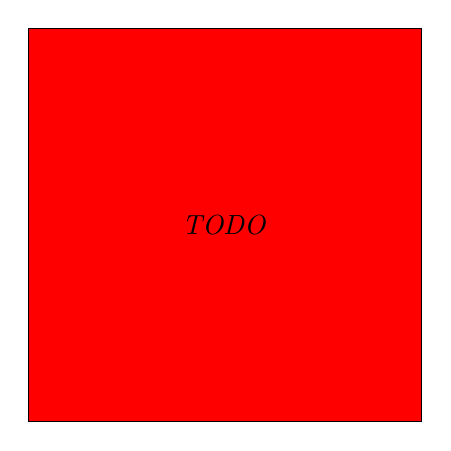
\begin{tikzpicture}
				\filldraw[fill=red] (0,0) rectangle (5,5) node[pos=.5] {\emph{TODO}};
			\end{tikzpicture}
		\end{center}
		Within the time interval \(\brackets*{t_n, t_{n + 1}}\) the waves may interact with one cell \(\brackets*{x_{j - \frac{1}{2}}, x_{j + \frac{1}{2}}}\), but should not reach the neighboring interface.
		This gives a time step constraint.
		If \(\lambda_p^{\parentheses*{j, n}} = \lambda_p\parentheses*{\bar{U}_j^n}, p = 1, \ldots, N\) denote the \emph{local} eigenvalues (i.e., characteristic speeds) of the flux Jacobian \(D_U F\) for the cell mean value \(\bar{U}_j^n\) in cell \(\brackets*{x_{j - \frac{1}{2}}, x_{j + \frac{1}{2}}}\), then for each cell the fastest wave should not reach the end of its cell:
		\[
			\max_{p = 1, \ldots, N}\absolute*{\lambda_p^{\parentheses*{j, n}}}\Delta t \le \Delta x.
		\]
		The fastest speed in the entire grid is \(\lambda^{\text{max}, \parentheses*{n}} := \max_{j \in \text{grid}}\parentheses*{\max_{p = 1, \ldots, N}\absolute*{\lambda_p^{\parentheses*{j, n}}}}\) and the global constraint thus reads
		\[
			\frac{\lambda^{\text{max}, \parentheses*{n}}\Delta t}{\Delta x} \le 1,
		\]
		which is analogous to the CFL condition.
		\item We have seen that the solution of the Riemann problem is constant along rays form the origin (\(\frac{x}{t} = \text{const.}\)), in particular, along \(x = 0\), which can be viewed as corresponding to the cell interface \(x_{j + \frac{1}{2}}\).
		Let \(U_L := \bar{U}_j^n\) and \(U_R := \bar{U}_{j + 1}^n\).
		Then we find
		\[
			U^*\parentheses*{U_L, U_R} := U^*\parentheses*{x_{j + \frac{1}{2}}, t; U_L, U_R} = \text{const.}
		\]
		and we obtain the \emph{Gondunov flux} in this case as
		\[
			\tilde{F}_{j + \frac{1}{2}}^n\parentheses*{U_L, U_R} = \frac{1}{\Delta t}\int_{t_n}^{t_{n + 1}}F\parentheses*{U^*\parentheses*{U_L, U_R}}\d t = F\parentheses*{U^*\parentheses*{U_L, U_R}}.
		\]
		However, this representation might be computationally expensive for nonlinear equations, since one has to find \(U^*\).
	\end{enumerate}
\end{remark}

\begin{example}[Godunov flux for linear systems]
	Let's consider a linear system with \(F\parentheses*{U} = AU\) where \(A \in \R^{N \times N}\) with eigenvalues \(\lambda_p\) and eigenvectors \(r_p, p = 1, \ldots, N\).
	For the Riemann problem with an initial condition given by a jump from \(U_L\) to \(U_R\) at the interface \(x_{j + \frac{1}{2}}\), we know from Theorem \ref{thm:10-7} that if the initial jump is decomposed as
	\[
		U_R - U_L = \sum_{p = 1}^N \alpha_p r_p,
	\]
	based on the jump sizes \(\alpha_p \in \R\), then the solution to the Riemann problem reads
	\[
		U^*\parentheses*{x, t; U_L, U_R} = U_L + \sum_{\lambda_p < \frac{x - x_{j + \frac{1}{2}}}{t}}\alpha_p r_p = U_R - \sum_{\lambda_p > \frac{x - x_{j + \frac{1}{2}}}{t}}\alpha_p r_p,
	\]
	which needs to be evaluated at \(x = x_{j + \frac{1}{2}}\) for the numerical flux.
	Hence the first expression gives
	\begin{align*}
		\tilde{F}_{j + \frac{1}{2}}\parentheses*{U_L, U_R} &= F\parentheses*{U^*\parentheses*{x_{j + \frac{1}{2}}, t; U_L, U_R}}\\
		&= AU_L + \sum_{\lambda_p < 0}\alpha_p Ar_p\\
		&= AU_L + \sum_{\lambda_p < 0}\alpha_p \lambda_p r_p,
	\end{align*}
	while the second yields
	\[
		\tilde{F}_{j + \frac{1}{2}}\parentheses*{U_L, U_R} = AU_R - \sum_{\lambda_p > 0}\alpha_p \lambda_p r_p
	\]
	accordingly.
	Next, we introduce \(\parentheses*{\lambda_p}^- := \min\parentheses*{\lambda_p, 0}\) as well as \(\parentheses*{\lambda_p}^+ := \max\parentheses*{\lambda_p, 0}\), and, using the matrix decomposition \(A = T^{-1}\Lambda T\) with \(\Lambda = \diag\parentheses*{\lambda_1, \ldots, \lambda_N}\), the matrices
	\[
		A^\pm = T^{-1}\Lambda^\pm T, \quad \text{where} \quad \Lambda^\pm = \diag\parentheses*{\parentheses*{\lambda_1}^\pm, \ldots, \parentheses*{\lambda_N}^\pm}.
	\]
	Then we find
	\[
		\tilde{F}_{j + \frac{1}{2}}\parentheses*{U_L, U_R} = AU_L + \sum_{p = 1}^N \alpha_p \parentheses*{\lambda_p}^- r_p = AU_L + A^- \parentheses*{U_R - U_L}
	\]
	and analogously
	\[
		\tilde{F}_{j + \frac{1}{2}}\parentheses*{U_L, U_R} = AU_R - A^+ \parentheses*{U_R - U_L}.
	\]
	Consequently, we obtain
	\[
		\tilde{F}_{j + \frac{1}{2}}\parentheses*{U_L, U_R} = \frac{1}{2}A\parentheses*{U_R + U_L} - \frac{1}{2}\absolute*{A}\parentheses*{U_R - U_L},
	\]
	where we have used the matrix modulus:
	\[
		\absolute*{A} = A^+ - A^- = T^{-1}\absolute*{\Lambda}T, \quad \absolute*{\Lambda} = \diag\parentheses*{\absolute*{\lambda_1}, \ldots, \absolute*{\lambda_N}}.
	\]
	The complete FV update therefore reads
	\begin{align*}
		\bar{U}_j^{n + 1} &= \bar{U}_j^n + \frac{\Delta t}{\Delta x}\parentheses*{\tilde{F}_{j - \frac{1}{2}}^n - \tilde{F}_{j + \frac{1}{2}}^n}\\
		&= \bar{U}_j^n + \frac{\Delta t}{\Delta x}A^+ \parentheses*{\bar{U}_{j - 1}^n - \bar{U}_j^n} + \frac{\Delta t}{\Delta x}A^- \parentheses*{\bar{U}_j^n - \bar{U}_{j + 1}^n},
	\end{align*}
	which is upwinding separately for the left- and right-moving waves.
	Alternatively, the update can be written as
	\[
		\bar{U}_j^{n + 1} = \bar{U}_j^n + \frac{\Delta t}{2\Delta x}A\parentheses*{\bar{U}_{j - 1}^n - \bar{U}_{j + 1}^n} + \frac{\Delta t}{2\Delta x}\absolute*{A}\parentheses*{\bar{U}_{j - 1}^n - 2\bar{U}_j^n + \bar{U}_{j + 1}^n},
	\]
	which resembles Lax-Wendroff, but with different diffusion.
\end{example}


\subsection{Approximate Riemann solver}

Unless the conservation law is linear, solving the local Riemann problems at each interface can be very costly in practice.
It thus seems desirable to use an approximation.

\begin{definition}[Approximate Riemann solver]\label{def:12-11}
	An \emph{approximate Riemann solver} considers a simplified flux function \(\hat{F}^{\parentheses*{j + \frac{1}{2}}}: \R^N \to \R^N\) at each grid cell interface \(x_{j + \frac{1}{2}}\) and solves the local Riemann problems for the equations
	\[
		\partial_t U + \partial_x \hat{F}^{\parentheses*{j + \frac{1}{2}}}\parentheses*{U} = 0
	\]
	instead.
	The final numerical flux for the FV-update can then be chosen as one of the following
	\begin{enumerate}
		\item \(\tilde{F}_{j + \frac{1}{2}}\parentheses*{U_L, U_R} = \hat{F}^{\parentheses*{j + \frac{1}{2}}}\parentheses*{\hat{U}^*\parentheses*{U_L, U_R}} - \hat{F}^{\parentheses*{j + \frac{1}{2}}}\parentheses*{U_L} + F\parentheses*{U_L}\),
		\item \(\tilde{F}_{j + \frac{1}{2}}\parentheses*{U_L, U_R} = \hat{F}^{\parentheses*{j + \frac{1}{2}}}\parentheses*{\hat{U}^*\parentheses*{U_L, U_R}} - \hat{F}^{\parentheses*{j + \frac{1}{2}}}\parentheses*{U_R} + F\parentheses*{U_R}\),
		\item \(\tilde{F}_{j + \frac{1}{2}}\parentheses*{U_L, U_R} = F\parentheses*{\hat{U}^*\parentheses*{U_L, U_R}}\),
	\end{enumerate}
	where \(\hat{U}^* \equiv \hat{U}_{j + \frac{1}{2}}^*\) is the \emph{approximate Riemann solution} at cell interface \(x_{j + \frac{1}{2}}\).
\end{definition}

\begin{remark}
	\begin{enumerate}
		\item All these numerical fluxes are consistent, in the sense that \(\tilde{F}\parentheses*{U, U} = F\parentheses*{U}\), and also Lipschitz-continuous.
		\item The versions (i) and (ii) are often simpler, because the Riemann solution is only used in the approximate flux function.
		But they may not yield the same result.
	\end{enumerate}
\end{remark}

A natural question now is, how to select a simplified flux?

\begin{definition}[Linear approximate Riemann solver]
	A \emph{linear approximate Riemann solver} for the flux function \(F\parentheses*{U}\) at cell interface \(x_{j + \frac{1}{2}}\) is given by
	\[
		\hat{F}^{\parentheses*{j + \frac{1}{2}}}\parentheses*{U} = \hat{A}\parentheses*{U_L, U_R}U
	\]
	with a suitable matrix function \(\hat{A}: \R^N \times \R^N \to \R^{N \times N}\), if
	\begin{enumerate}
		\item the matrix \(\hat{A}\parentheses*{U_L, U_R}\) is diagonalizable with real eigenvalues, for all relevant \(U_L, U_R \in \R^N\), and
		\item the matrix \(\hat{A}\parentheses*{U, U}\) is a ``reasonable'' approximation to the Jacobian \(D_U F\parentheses*{U}\).
	\end{enumerate}
\end{definition}

\begin{theorem}[Roe-solver]
	If we choose the matrix \(\hat{A}\) such that
	\[
		\hat{A}\parentheses*{U_L, U_R}\parentheses*{U_R - U_L} = F\parentheses*{U_R} - F\parentheses*{U_L}
	\]
	at the cell interface \(x_{j + \frac{1}{2}}\), then the matrix is called \emph{Roe-matrix} and the numerical fluxes (i), (ii), (iii) given in Definition \ref{def:12-11} are identical to
	\[
		\tilde{F}_{j + \frac{1}{2}}\parentheses*{U_L, U_R} = F\parentheses*{U_L} + \hat{A}\parentheses*{U_L, U_R}^- \parentheses*{U_R - U_L} = F\parentheses*{U_R} - \hat{A}\parentheses*{U_L, U_R}^+ \parentheses*{U_R - U_L}.
	\]
\end{theorem}

\begin{proof}
	The identity of the fluxes (i), (ii), (iii) follows from
	\begin{align*}
		\tilde{F}\parentheses*{U_L, U_R} &= \hat{F}^{\parentheses*{j + \frac{1}{2}}}\parentheses*{\hat{U}^*} - \hat{F}^{\parentheses*{j + \frac{1}{2}}}\parentheses*{U_L} + F\parentheses*{U_L}\\
		&= \hat{A}\parentheses*{\hat{U}^* - U_L} + F\parentheses*{U_L}\\
		&= F\parentheses*{\hat{U}^*} - F\parentheses*{U_L} + F\parentheses*{U_L}\\
		&= F\parentheses*{\hat{U}^*}
	\end{align*}
	using the Roe-matrix property, and reversing the argument
	\begin{align*}
		\tilde{F}\parentheses*{U_L, U_R} &= F\parentheses*{\hat{U}^*} - F\parentheses*{U_R} + F\parentheses*{U_R}\\
		&= \hat{F}^{\parentheses*{j + \frac{1}{2}}}\parentheses*{\hat{U}^*} - \hat{F}^{\parentheses*{j + \frac{1}{2}}}\parentheses*{U_R} + F\parentheses*{U_R}.
	\end{align*}
	Furthermore, the flux
	\[
		\hat{F}^{\parentheses*{j + \frac{1}{2}}}\parentheses*{\hat{U}^*} = \hat{A}\hat{U}^*
	\]
	is nothing but the linear Godunov flux from the example above.
\end{proof}

\begin{remark}
	\begin{enumerate}
		\item A Roe-matrix must be constructed for a concrete system of conservation laws separately.
		Typically, it has the form
		\[
			\hat{A}\parentheses*{U_L, U_R} = D_U F\parentheses*{U^{\parentheses*{\text{avg}}}\parentheses*{U_L, U_R}}
		\]
		for some \emph{average state} \(U^{\parentheses*{avg}}\).
		\item The Roe solver remains expensive, because at every interface the matrix \(\hat{A}\) must be build (i.e., assembled) and its complete Eisner system computed.
	\end{enumerate}
\end{remark}

\begin{example}[Local Lax-Friedrichs flux]
	It also makes sense to consider the averaged numerical flux
	\[
		\tilde{F}_{j + \frac{1}{2}}\parentheses*{U_L, U_R} = \frac{1}{2}\parentheses*{F\parentheses*{U_L} + F\parentheses*{U_R}} - \frac{1}{2}\absolute*{\hat{A}}\parentheses*{U_R - U_L},
	\]
	where
	\[
		\absolute*{\hat{A}}\parentheses*{U_R - U_L} = \sum_{p = 1}^N \alpha_p \absolute*{\hat{\lambda}_p}\hat{r}_p, \quad \text{with} \quad \sum_{p = 1}^N \alpha_p \hat{r}_p = U_R - U_L.
	\]
	This can be further simplified by using the maximal eigenvalue
	\[
		\sum_{p = 1}^N \alpha_p \absolute*{\hat{\lambda}_p}\hat{r}_p \approx \lambda^\text{max} \sum_{p = 1}^N \alpha_p \hat{r}_p = \lambda^\text{max} \parentheses*{U_R - U_L},
	\]
	which then yields the numerical flux
	\[
		\tilde{F}_{j + \frac{1}{2}}\parentheses*{U_L, U_R} = \frac{1}{2}\parentheses*{F\parentheses*{U_L}, F\parentheses*{U_R}} - \frac{1}{2}\lambda^\text{max} \parentheses*{U_R - U_L}.
	\]
	This flux is called \emph{local Lax-Friedrichs flux}.
	The maximal speed \(\lambda^\text{max}\) has to be estimated from the local Jacobian \(D_U F\parentheses*{U}\) between \(U_L\) and \(U_R\).
\end{example}
